La prima fase dell'algoritmo si occupa dato un dataset avente traiettorie \(n\)-dimensionali di generare un set di quanti distinti e di esprimere le traiettorie come combinazioni di questi.
Lo scopo di questa fase è quello di esprimere le traiettorie in un sistema di riferimento custom univoco per tutto il dataset.
Tramite questa trasformazione dovrà essere possibile determinare la vicinanza di due traiettorie in maniera univoca.
Inoltre i quanti di cui dovrà essere composto questo sistema dovranno essere di molto inferiori rispetto al numero di traiettorie.
Questa compressione dell'informazione sarà fondamentale per le fasi successive, in particolare per quella di ricerca degli itemset.

Punto focale di questa prima fase è il sistema di riferimento fornito in input.
Questo specifica quante e quali dimensioni considerare all'interno del problema.
All'interno del sistema è presente l'insieme dei valori che la singola dimensione può assumere.
La definizione dei quanti avviene quindi sulla base dei singoli valori possibili di ogni dimensione.
Date \(n\) dimensioni utilizzate, lo spazio di ricerca composto da tutte le traiettorie proiettate sulle \(n\) dimensioni è suddiviso in un insieme di quanti.
Un quanto per definizione è rappresentabile come un ipercubo \(n\) dimensionale avente un id univoco all'interno dell'insieme.
Ogni quanto è caratterizzato da uno specifico valore per ciascuna delle \(n\) dimensioni e intuitivamente copre una parte dello spazio totale di ricerca.
Una traiettoria può essere espressa utilizzando il set di quanti sopra definito.
Ogni punto di una traiettoria infatti individua uno specifico quanto.
Le traiettorie passano così dall'essere insiemi di punti a insiemi di quanti univoci per tutto il set di traiettorie.
Intuitivamente due punti risulteranno vicini quando apparterranno allo stesso quanto.
Una volta terminata la conversione, la prima fase dell'algoritmo può dirsi conclusa.

Trattando del caso specifico della ricerca dei pattern di co-movimento, quanto detto sopra viene declinato come segue:
Si utilizza un sistema di riferimento tridimensionale, basato su latitudine, longitudine e tempo.
I quanti sono definiti mediante un mapping su griglia, che produce cubi omogenei.
Questi cubi sono chiamati celle. 

Ogni cella avrà una componente spaziale e una temporale.
L'area spaziale coperta da una cella è determinata dal parametro \(s\) ed è espressa in metri rispetto alle coordinate polari di ogni punto.

Per quanto riguarda la dimensione temporale \(t\) invece sono prese in considerazione nello specifico due scale cicliche: ore del giorno, giorni della settimana.
Rispetto a una metrica di tempo monotona basata su data e ora di ogni singolo punto, come ad esempio in SPARE, una scala circolare ha due vantaggi: il primo riguarda
il supporto a pattern ciclici che verrebbero altrimenti ignorati e in secondo luogo il ridotto range di valori della scala (da 0 a 23 in caso di scala giornaliera, da 0 a 6 in quella settimanale) previene l'esplosione nel numero di celle al crescere del dataset.

Una volta determinata il lato spaziale delle celle e la loro durata temporale, viene generato l'insieme delle celle \textit{C}. 
Ottenuto questo, è necessario per concludere questa prima fase esprimere ogni traiettoria nella nuova formulazione.
Così facendo una traiettoria non sarà più definita come la composizione di diversi punti isolati nel tempo, ma come un insieme di celle. 
La~\cref{fig:chap-3:trajectory-cell-division} mostra un esempio di conversione in un sistema di riferimento basato su celle:

\begin{figure}
  \centering
  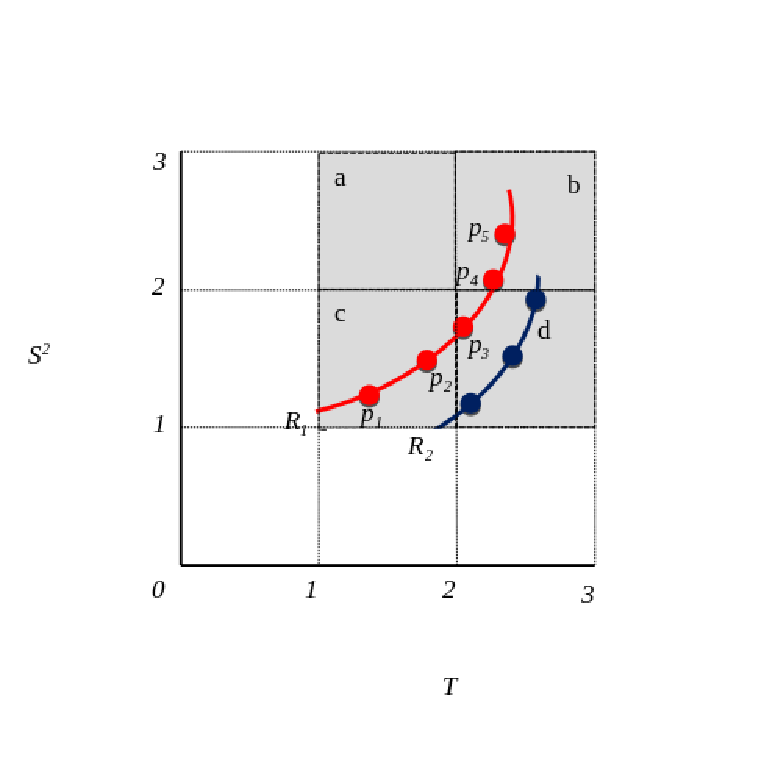
\includegraphics[scale=.8]{/sec-3/TrajectoryCellDecomposition.pdf}
  \caption{Mapping di due traiettorie, \(R_1, R_2\)in un sistema di riferimento basato su celle. Sugli assi x e y sono espressi latitudine e longitudine, il tempo invece è espresso in pedice ai punti}%
  \label{fig:chap-3:trajectory-cell-division}
\end{figure}

Prendendo in considerazione le traiettorie \(R_1, R_2\), è possibile vedere come i punti \(p_1,p_2\) appartengano alla cella \(c\),
\(p_3\) a \(d\) mentre \(p_4,p_5\) a \(b\); analogamente ogni punto della traiettoria \(R_2\) sia attribuibile a \(d\).
Il set di celle del problema sarà quindi composto dalle seguenti celle: \(\langle b,c,d \rangle\) mentre le due traiettorie saranno espresse in funzione del nuovo sistema di riferimento come segue:

\begin{itemize}

  \item \(R_1\). \(\langle b,c,d \rangle\)
  \item \(R_2\). \(\langle d \rangle\)

\end{itemize}

Va sottolineato infine che, sebbene appaia nell'immagine, la cella \(a\) non viene effettivamente generata, poiché nessuna traiettoria ha un punto entro i suoi confini.

Una volta che le traiettorie sono state espresse nelle nuove coordinate, questo primo passo dell'algoritmo giunge a termine.

La scelta delle dimensioni di ogni cella influenza molto i passaggi successivi. 
Celle piccole produrranno traiettorie lunghe, estendendo il possibile spazio di ricerca di ogni cluster.
Tanto più ampio lo spazio di ricerca, tanto più a lungo dura la sua esplorazione, tuttavia è possibile eseguire una ricerca più fine su di esso.
Lati spaziali più ampli e dimensioni temporali ridotte generano celle più grandi, con uno spazio di ricerca più ridotto e risultati più grezzi.